% Chapter 4: Experimental Procedure 
\chapter{Appendices}
\label{chapter:appendices}

\graphicspath{ {report/Appendices/assets/} } 

% \setlength{\voffset}{0cm}
% \setlength{\hoffset}{0cm}

\section{Firmware Implementations}
\label{app:firmware}

\begin{listing}[!htb]
\footnotesize
\begin{minted}{python}
from ulab import numpy as np

def power_iteration(A, iterations):
    """
    Iterative algo. to find the eigenvector of a matrix A corresponding to the largest
    eigenvalue.
    """
    # choose random initial vector to reduce risk of choosing one orthogonal to 
    # target eigen vector
    b_k = np.array([urandom.random() for i in range(len(A))])

    for _ in range(iterations):
        b_k1 = np.dot(A, b_k)
        b_k1_norm = np.linalg.norm(b_k1)
        # re normalize the vector
        b_k = b_k1 / b_k1_norm

    return b_k1_norm, b_k

\end{minted}
\caption{MicroPython implementation of the Power Iteration algorithm presented in Algorithm \ref{alg:power-iteration} for finding the maximum real eigenvalue of a symmetric, real-valued matrix}
\label{app-listing:power-iteration-mpy}
\end{listing}

\begin{listing}[!htb]
\footnotesize
\begin{minted}{python}
from ulab import numpy as np

def qr_iteration(A, iterations=30):
    
    """
    Use the QR iteration algorithm to iteratively solve for the eigenvectors and eigenvalues
    of a matrix A. Note: only guaranteed to recover exactly for symmetric matrices
    with real eigenvalues. May work partially for asymmetric matrices (no complex support yet).
    
    Number of iterations is specified by `iterations` and should be tuned empirically. Typically,
    30 is more than enough.
    Returns:
        `lam`: vector of eigenvalues
        `Q_bar`: matrix of eigenvectors (columns)
    """

    Ak = A
    Q_bar = np.eye(len(Ak))

    for _ in range(iterations):
        Qk, Rk = np.linalg.qr(Ak)
        Ak = np.dot(Rk, Qk)
        Q_bar = np.dot(Q_bar, Qk)

    lam = np.diag(Ak)
    return lam, Q_bar

\end{minted}
\caption{MicroPython implementation of the QR Iteration algorithm presented in Algorithm \ref{alg:qr-iteration}}
\label{app-listing:qr-iteration-mpy}
\end{listing}

\begin{listing}[h]
\footnotesize
\begin{minted}{python}
from ulab import numpy as np

def solve_gen_eig_prob(A, B, eps=1e-6):
    """
    Solves the generalised eigenvalue problem of the form:
    Aw = lambda*Bw
    
    Note: can be validated against `scipy.linalg.eig(A, b=B)`
    
    Ref: 
    'Eigenvalue and Generalized Eigenvalue Problems: Tutorial (2019)'
    Benyamin Ghojogh and Fakhri Karray and Mark Crowley
    arXiv 1903.11240

    """
    Lam_b, Phi_b = np.linalg.eig(B) # eig decomp of B alone
    Lam_b = np.eye(len(Lam_b))*Lam_b # convert to diagonal matrix of eig vals
    
    Lam_b_sq = replace_nan(Lam_b**0.5)+np.eye(len(Lam_b))*eps
    Phi_b_hat = np.dot(Phi_b, np.linalg.inv(Lam_b_sq))
    A_hat = np.dot(np.dot(Phi_b_hat.transpose(), A), Phi_b_hat)
    Lam_a, Phi_a = np.linalg.eig(A_hat)
    Lam_a = np.eye(len(Lam_a))*Lam_a
    
    Lam = Lam_a
    Phi = np.dot(Phi_b_hat, Phi_a)
    
    return np.diag(Lam), Phi

\end{minted}
\caption{MicroPython implementation of the generalised eigenvalue algorithm in Algorithm \ref{alg:gen-eig-algo}}
\label{app-listing:gen-eig-prob-mpy}
\end{listing}

\begin{listing}[h]
\footnotesize
\begin{minted}{python}
from ulab import numpy as np

class CCA():
    """
    Canonical Correlation Analysis algorithm for SSVEP decoding. Reference 
    signal `Y` is a harmonic reference set with `Nh` harmonics.
    
    Expects a list of `stim_freqs` corresponding to SSVEP stimulus frequencies.
    Requires sampling frequncy `fs` for the harmonic ref.
    """
    
    def __init__(self, stim_freqs, fs, Nh=2):
        self.Nh = Nh
        self.stim_freqs = stim_freqs
        self.fs = fs
        
    def compute_corr(self, X_test):            
        result = {}
        Cxx = np.dot(X_test, X_test.transpose()) # precompute data auto correlation matrix
        for f in self.stim_freqs:
            Y = harmonic_reference(f, self.fs, np.max(X_test.shape), Nh=self.Nh, standardise_out=False)
            rho = self.cca_eig(X_test, Y, Cxx=Cxx) # canonical variable matrices. Xc = X^T.W_x
            result[f] = rho
        return result
    
    @staticmethod # define as static to allow non-CCA instances to use this func
    def cca_eig(X, Y, Cxx=None, eps=1e-6):
        if Cxx is None:
            Cxx = np.dot(X, X.transpose()) # signal covariance matrix
        Cyy = np.dot(Y, Y.transpose())  # reference covariance matrix
        Cxy = np.dot(X, Y.transpose()) # cross covariance matrix
        Cyx = np.dot(Y, X.transpose()) # same as Cxy.T

        M1 = np.dot(np.linalg.inv(Cxx+eps), Cxy) # intermediate result
        M2 = np.dot(np.linalg.inv(Cyy+eps), Cyx)

        lam, _ = solve_eig_qr(np.dot(M1, M2), 20) # solve eig. vals using QR iteration
        return np.sqrt(lam)

\end{minted}
\caption{MicroPython implementation of the CCA algorithm from Algorithm \ref{alg:cca}}
\label{app-listing:cca-algo}
\end{listing}

\begin{listing}[h]
\footnotesize
\begin{minted}{python}
from ulab import numpy as np

class UnivariateMsetCCA():
    """
    Multiset CCA algorithm for SSVEP decoding.
    
    Computes optimised reference signal set based on historical observations
    and uses ordinary CCA for final correlation computation given a new test
    signal.
    
    Note: this is a 1 channel implementation (Nc=1)
    """
    
    def __init__(self):
        self.Ns, self.Nt = None, None
        
    def fit(self, X, compress_ref=True):
        """
        Expects a training matrix X of shape Nt x Ns. If `compress_ref=True`, the `Nt` components
        in optimised reference signal Y will be averaged to form a single reference vector. This
        can be used for memory optimisation but will likely degrade performance slightly.         
        """
        if X.shape[0] > X.shape[1]:
            print("Warning: received more trials than samples. This is unusual behaviour: check X")
        R = np.dot(X, X.transpose()) # inter trial covariance matrix
        S = np.eye(len(R))*np.diag(R) # intra-trial diag covariance matrix

        lam, V = solve_gen_eig_prob((R-S), S) # solve generalised eig problem
        w = V[:, np.argmax(lam)] # find eigenvector corresp to largest eigenvalue
        Y = np.array([x*w[i] for i, x in enumerate(X)]) # store optimised reference vector Nt x Ns
        self.Y  = Y
        if compress_ref:
            self.Y = np.mean(Y, axis=0).reshape((1, max(Y.shape))) # this will average Nt components in Y: Nc x Nt -> 1 x Nt
        
    def compute(self, X_test):
        if self.Y is None:
            raise ValueError("Reference matrix Y must be computed using `fit` before computing corr")
        if len(X_test.shape) == 1:
            X_test = X_test.reshape((1, len(X_test)))
        return CCA.cca_eig(X_test, self.Y)[0] # use ordinary CCA with optimised ref. Y

\end{minted}
\caption{MicroPython implementation of the MsetCCA algorithm from Algorithm \ref{alg:mset-cca}}
\label{app-listing:mcca-algo}
\end{listing}

\begin{listing}[h]
\footnotesize
\begin{minted}{python}
from ulab import numpy as np

class GCCA():
    """
    Generalised canonical component analysis.
    
    Expects the target frequency at `f_ssvep`. `fs` is the sampling rate used and `Nh` the number of harmonics for the harmonic reference signal. 
    
    Ref: 'Improving SSVEP Identification Accuracy via Generalized Canonical Correlation Analysis'
    Sun, Chen et al
    """
    
    def __init__(self, f_ssvep, fs, Nh=3, name=None):
        self.Nc, self.Ns, self.Nt = None, None, None
        self.Nh = Nh
        self.w_chi_bar_n = None
        self.w_Y_n = None
        self.w_Chi_n = None
        self.fs = fs
        self.f_ssvep = f_ssvep
        
        self.name = name or "gcca_{0}hz".format(f_ssvep)
            
        
    def fit(self, X):
        """
        Fit against training tensor X.
        
        X should be a 3rd order tensor of dim (Nc x Ns x Nt)
        """
        assert len(X.shape) == 3, "Expected 4th order input data tensor: Nc x Ns x Nt"
        self.Nc, self.Ns, self.Nt = X.shape
        
        Chi_n = X
        Chi_n_c = Chi_n.reshape((self.Nc, self.Ns*self.Nt))

        Chi_bar_n = np.mean(Chi_n, axis=-1) # mean over trials for each channel with all samples: output shape is Nc x Ns x 1
        Chi_bar_n_c = np.concatenate([Chi_bar_n for i in range(self.Nt)], axis=1) # concat along columns

        Y_n = cca_reference([self.f_ssvep], self.fs, self.Ns, Nh=self.Nh).reshape(-1, self.Ns)
        Y_n_c = np.concatenate([Y_n for i in range(self.Nt)], axis=1)

        # form X and D and find eigenvals
        X = np.c_[Chi_n_c.T, Chi_bar_n_c.T, Y_n_c.T].T

        d1 = Chi_n_c.dot(Chi_n_c.T)
        d2 = Chi_bar_n_c.dot(Chi_bar_n_c.T)
        d3 = Y_n_c.dot(Y_n_c.T)
        D = block_diag(d1, d2, d3)

        lam, W_eig = solve_gen_eig_prob(X.dot(X.T), D) # solve generalised eigenvalue problem

        i = np.argmax(np.real(lam))
        w = W_eig[:, i] # optimal spatial filter vector with dim (2*Nc + 2*Nh)
        
        w_Chi_n = w[:self.Nc] # first Nc weight values correspond to data channels
        w_Chi_bar_n = w[self.Nc:2*self.Nc] # second Nc weights correspond to Nc template channels
        w_Y_n = w[2*self.Nc:] # final 2*Nh weights correspond to ref sinusoids with harmonics
        
        self.w_chi_bar_n =  w_Chi_bar_n.T.dot(Chi_bar_n)
        self.w_Y_n = w_Y_n.T.dot(Y_n)
        self.w_Chi_n = w_Chi_n
            
    def compute(self, X_test):
        if self.w_chi_bar_n is None:
            raise ValueError("call `.fit(X_train)` before performing classification.")

        rho1 = correlation(self.w_Chi_n.T.dot(X_test), self.w_chi_bar_n)[0]
        rho2 = correlation(self.w_Chi_n.T.dot(X_test), self.w_Y_n)[0]

        return np.sum([np.sign(rho_i)*rho_i**2 for rho_i in [rho1, rho2]])

\end{minted}
\caption{Python implementation of the GCCA algorithm from Algorithm \ref{alg:gcca}}
\label{app-listing:gcca-algo}
\end{listing}

% \setlength{\voffset}{-2.54cm}
% \setlength{\hoffset}{-2.54cm}

\section{EEG Hardware Schematics}

\label{appendix:schematics}
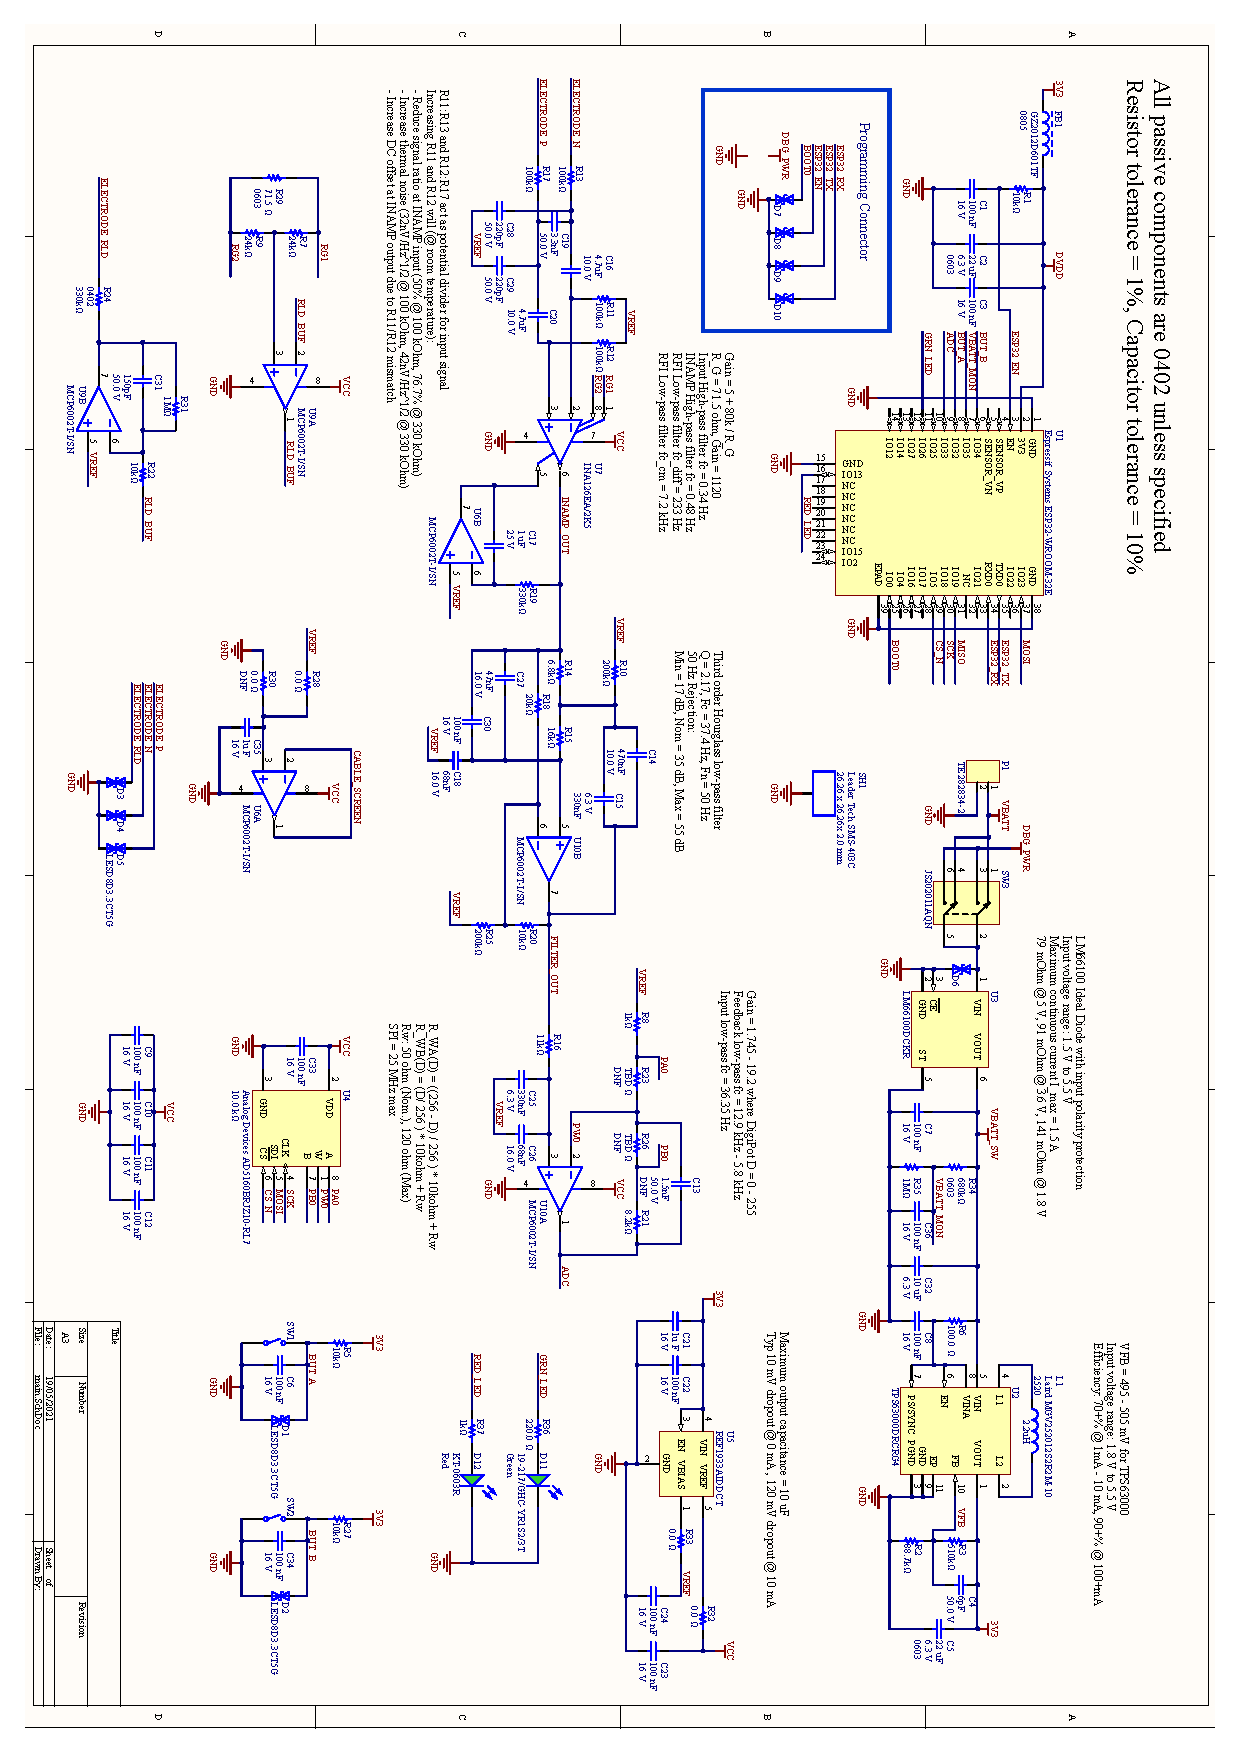
\includepdf[pages=-]{schematic.PDF}
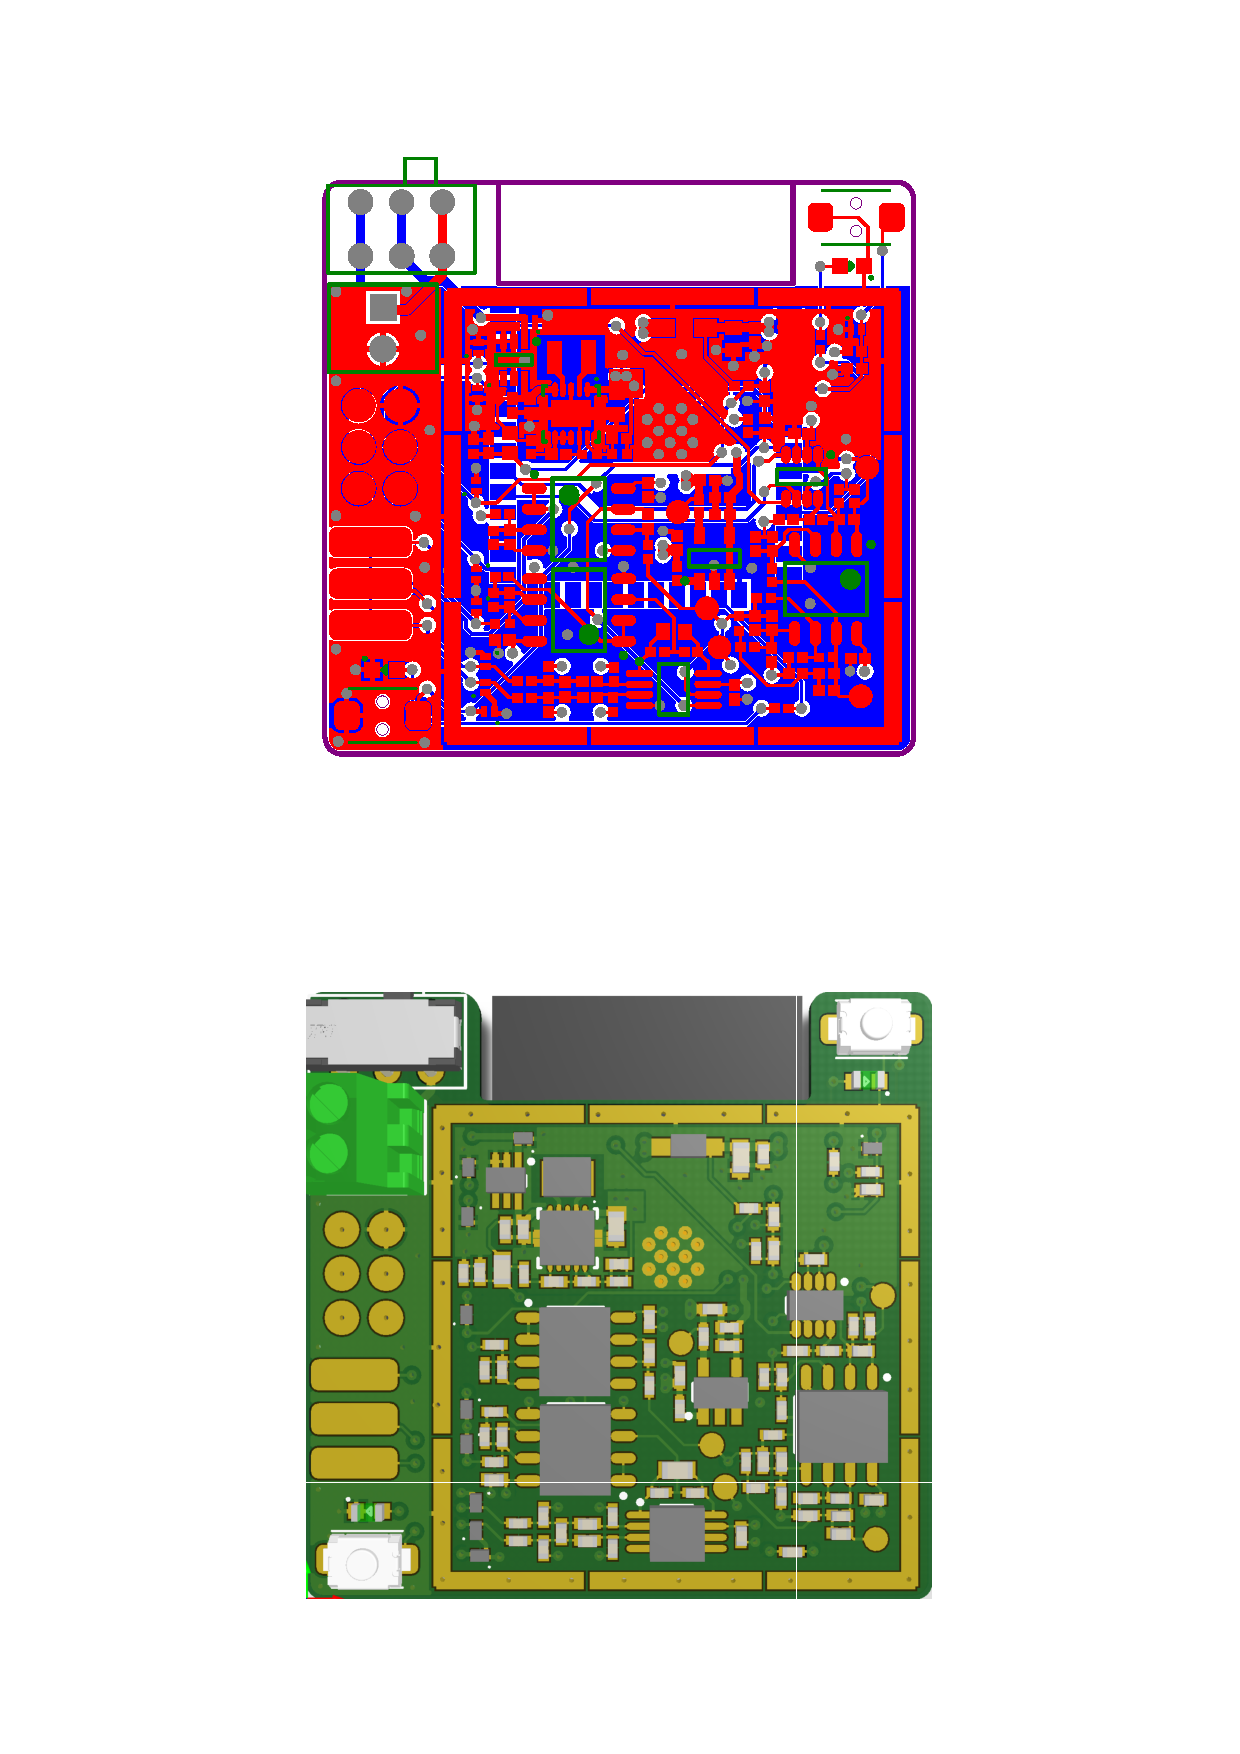
\includepdf[pages=-]{board-layouts.PDF}